\newline
\newline
\title{LEZIONE 11 26/03/2020}\newline
\textbf{link} \href{https://web.microsoftstream.com/video/55dca95e-fe7f-4bf2-82e6-d3024939e5c3?list=user&userId=faa91214-a6f5-40d7-8875-253fd49b8ce1}{clicca qui} [registrazione solo audio, no video]\newline
\newline
Questa realizzazione è sempre raggiungibile, infatti usando questi $(A,b,c,d)$, la matrice di raggiungibilità ha la seguetne forma:
\[
    M_R = \left[\begin{matrix}
        0     & 0     & \dots & 0     & 1    \\
        0     & \dots & 0     & 1     & *    \\
        \dots & 0     & 1     & *     & \dots\\
        0     & 1     & *     & \dots & *    \\
        1     & *     & \dots & *     & *    \\
    \end{matrix}\right]
\]
Questa matrice è ovviamente non singolare.\newline
\newline
Infatti questo metodo di realizzazione prende il nome di \textbf{forma canonica di ragigungibilità}.\newline
\newline
Esiste anche la \textbf{forma canonica di osservabilità}: vedi libro, studio autonomo.\newline
\newline
Concetti fondamentali:
\begin{itemize}
    \item Partendo dalle matrici ($A,b,c,d$), esiste sempre una e una sola funzione di trasferimento $G(s)$, una e una sola matrice di raggiungibilità $M_R$, una e una sola matrice di osservabilità $M_O$. Quindi siamo a conoscenza dell'intero sistema.
    \item Se invece partiamo da una funzione di trasferimento senza cancellazioni, allora esistono infinite (a meno di una trasformazione di similarità) quaterne ($A,b,c,d$). Queste quaterne possono essere divise in due famiglie:
    \begin{itemize}
        \item Minime: in cui la dimensione di $A$ è uguale al grado della funzione di trasferimento $G(s)$; queste sono raggiungibili e osservabili, e non ci sono cancellazioni.
        \item Non minime: in cui esistono cancellazioni e possono essere o non raggiungibili (ma osservabili) o non osservabili (ma raggiungibili) o non raggiungibili e non osservabili.
    \end{itemize}
\end{itemize}
\subsection{Esempi}
\textbf{es.} Esempio di funzione di trasferimento con calcellazione, cioè con parte nascosta:
\[
    G(s) = \frac{(s+1) (s+2)}{(s+1)(s+3)(s+4))}
\]
Ci sarebbe da fare una semplificazione fra $(s+1)$ al numeratore e $(s+1)$ al denominatore. Però vediamo cosa succede se non facciamo la cancellazione:
\[
    G(s) = \frac{s^2 + 3s + 2}{s^3+8s^2 +19 s + 12}
\]
Scriviamo ora la forma canonica di raggiungibilità:
\[
    A= \left[\begin{matrix}
        0 & 1 & 0\\
        0 & 0 & 1\\
        -12 & -19 & -8
    \end{matrix}\right]; \;\;\;\;\;b = \left[\begin{matrix}
        0 \\0\\1
    \end{matrix}\right]; \;\;\;\;\; c=\left[\begin{matrix}
        2&3&1
    \end{matrix}\right]; \;\;\;\;\;d=0.
\]
Premettiamo che \textbf{la presenza di una cancellazione ci impone il fatto che la realizzazione ($A,b,c,d$) non può essere raggiungibile e osservabile contemporaneamente}. Quindi siccome abbiamo eseguito la realizzazione con la forma canonica di raggiungibilità, sicuramente $(A,b,c,d)$ sarà raggiungibile e di conseguenza non osservabile (perchè esiste una cancellazione). Se avessimo usato la forma canonica di osservabilità saremmo giunti a una realizzazione osservabile, ma non raggiungibile.\newline
\newline
\textbf{oss.} Errore tipico: Questo concetto è anche utilizzato nell'analisi di funzioni di trasferimento in cui sono presenti cancellazioni: se abbiamo valutato che è raggiungibile è inutile controllare se è anche osservabile, ovviamente non lo sarà! Vale anche il viceversa, cioè se abbiamo valutato che è osservabile, sicuramente non sarà raggiungibile. Da notare è che se si valuta la funzione di trasferimento non raggiungibile, bisogna per forza controllare se sia o meno osservabile! E anche il viceversa, cioè se valutiamo che è non osservabile, dobbiamo controllare se sia o meno raggiungibile! Potrebbe essere sia non osservabile sia non raggiungibile.
\newline
\newline
Quindi dalla sola funzione di trasferimento (con una parte nascosta) non possiamo sapere se il sistema è raggiungibile e osservabile (contemporaneamente), lo possiamo sapere solo dalle matrici. Se partiamo dalla funzione di trasferimento, le cancellazioni possono essere provocate o da una non raggiungibilità o da una non osservabilità, ma non sappiamo quale, quindi dobbiamo decidere se realizzare il sistema con la forma canonica osservabile o raggiungibile.
\newpage
\section{Sistemi interconnessi (LTI a TC)}
\subsection{Logica fondamentale degli schemi a blocchi}
Rappresentiamo i sistemi interconnessi (LTI a TC) con schemi a blocchi.\newline
\newline
Logica fondamentale dei sistemi interconnessi: 
\begin{center}
    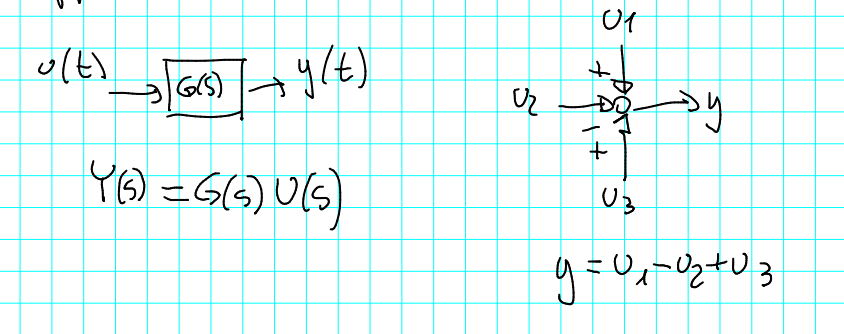
\includegraphics[height=3cm]{../lezione11/img1.PNG}
\end{center}
(a sinistra abbiamo una formula molto usata a destra nodo sommatore).\newline
\newline
Vediamo il seguente problema:\newline
[immagine dagli appunti del prof]
\begin{center}
    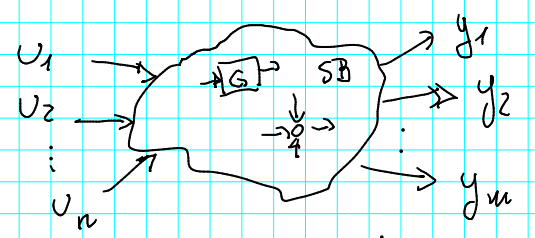
\includegraphics[height=3cm]{../lezione11/img2.PNG}
\end{center}
\ \newline
Ipotesi: tutti i blocchi sono privi di parti nascoste, ovvero tutte le loro funzioni di trasferimento hanno numeratore e donominatore coprimi (non ci sono cancellazioni).\newline
Domande:
\begin{itemize}
    \item Come calcolo la generica funzione di trasferimento da $Y_i(s)$ a $U_j(s)$?
    \item Che relazione c'è tra la stabilità delle singole funzioni di trasferimento e quella del sistema complessivo?
    \item Posto che i singoli blocchi non hanno parti nascoste, il sistema complessivo può averne?
\end{itemize}
\subsection{Elaborazione degli schemi a blocchi}
Andiamo a vedere tre configurazioni particolari che ci permettono di studiare gli schemi a blocchi.
\subsubsection{Blocchi in serie o cascata}
[immagine dagli appunti del prof]
\begin{center}
    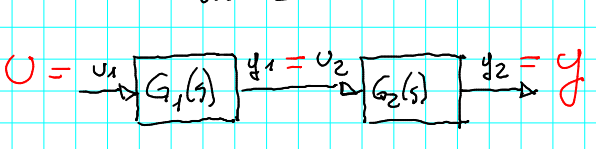
\includegraphics[height=3cm]{../lezione11/img3.PNG}
\end{center}
Quale è la funzione di trasferimento $\frac{Y(s)}{U(s)}$ per un blocco in serie?
\[
    Y= Y_2 = G_2U_2 = G_2 Y_1 = G_2G_1 U_1 = G_2G_1 U \Longrightarrow \frac{Y}{U} = G_2G_1
\]
Scriviamo ora $G_1 = \frac{N_1}{D_1}$ e $G_2= \frac{N_2}{D_2}$:
\[
    \Longrightarrow \frac{Y}{U} = G_2 G_1 = \frac{N_1N_2}{D_1D_2}
\]
Per ipotesi abbiamo detto che $N_i$ e $D_i$ sono coprimi fra di loro, ma non per forza lo sono anche $N_i$ e $D_j$.\newline
Quindi gli autovalori del sistema complessivo sono $\{\text{poli di $G_1$}\} U \{\text{poli di $G_2$}\}$, ma possono esserci cancellazioni tra $N_1$ e $D_2$ e/o tra $N_2$ e $D_1$.\newline
\newline
Di conseguenza:
\begin{itemize}
    \item $G_1$ e $G_2$ (entrambi) asintoticamente stabili è condizione neccessaria e sufficiente ($\Leftrightarrow$) per avere un sistema complessivo asintoticamente stabile.
    \item possono esserci cancellazioni, cioè parti nascoste.
\end{itemize} 
\ \newline
Vediamo ora la stesa cosa nello spazio di stato (realizzazione minime e quindi raggiungibili e osservabili).
Le equazioni costitutive dei blocchi sono:
\[
    G_1: \begin{cases}
        \dot{x}_1 = A_1 x_1 + b_1 u_1\\
        y_1 = c_1 x_1 + d_1 u_1
    \end{cases}; \;\;\;\;\;\;\;\;\;\;\;\;\;\;\;G_2 : \begin{cases}
        \dot{x}_2 = A_2 x_2 + b_2 u_2\\
        y_2 = c_2 x_2 + d_2 u_2
    \end{cases}
\]
Le equazioni di connessione sono:
\[
    u = u_1; \;\;\;\;\;\;\;\;\;\;y_1 = u_2 \;\;\;\;\;\;\;\;\;\;y=y_2
\]
Di conseguenza:
\[
    \begin{cases}
        \dot{x}_1 = A_1 x_1 + b_1 u\\
        \dot{x}_2 = A_2 x_2 + b_2 y_1 = A_2 x_2 + b_2 c_1x_1 + b_2 d_1 u_1\\
        y = c_2 x_2 + d_2 y_1 = c_2 x_2 + d_2 c_1 x_1 + d_2 d_1 u
    \end{cases}
\]
Che ci danno il sisetma matriciale nella forma:
\[
    \begin{cases}
        \left[\begin{matrix}
            \dot{x}_1\\\dot{x}_2
        \end{matrix}\right] = \left[\begin{matrix}
            A_1 & 0 \\ b_2 c_1 & A_2
        \end{matrix}\right] \left[\begin{matrix}
            x_1\\x_2
        \end{matrix}\right] + \left[\begin{matrix}
            b_1 \\b_2 d_1
        \end{matrix}\right] u\\
        y = \left[\begin{matrix}
            d_2c_1 & c_2
        \end{matrix}\right] \left[\begin{matrix}
            x_1\\x_2
        \end{matrix}\right] + d_1d_2 u
    \end{cases}
\]
\subsubsection{Blocchi in parallelo}
[immagine dagli appunti del prof]
\begin{center}
    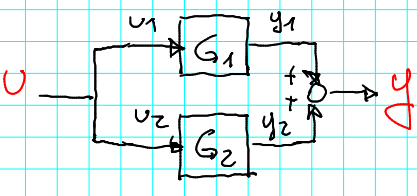
\includegraphics[height=3cm]{../lezione11/img4.PNG}
\end{center}
\[
    Y = Y_1 + Y_2 = G_1 U_1 + G_2 U_2 = (G_1 + G_2)U \Longrightarrow \frac{Y}{U} = G_1 +G_2
\]
scrivendo $G_i= \frac{N_i}{D_i}$
\[
    \Longrightarrow \frac{Y}{U} = \frac{N_1}{D_1} + \frac{N_2}{D_2} = \frac{N_2 D_1 + N_1 D_2}{D_1D_2}
\]
Gli autovalori del complessivo sistema sono $\{\text{poli di $G_1$}\} U \{\text{poli di $G_2$}\}$:
\begin{itemize}
    \item $G_1$ e $G_2$ (entrambi) asintoticamente stabili è condizione necessaria e sufficiente ($\Leftrightarrow$) per avere un sistema complessivo asintoticamente stabile.
    \item possono esserci cancellazioni, cioè parti nascoste (ce ne sono di sicuro se $D_1$ e $D_2$ non sono coprimi).
\end{itemize}
\ \newline
Vediamo questo ragionamento applicato allo spazio di stato:\newline
Equazioni costituitive dei blocchi:
\[
    G_1 : (A_1, b_1, c_1,d_1); \;\;\;\;\;\;\;\;\;\;\;\;\;\;\; G_2 : (A_2, b_2,c_2,d_2).
\]
Equazioni di connessione:
\[
    u_1 = u; \;\;\;\;\;\;\;\;\;\; u_2 = u \;\;\;\;\;\;\;\;\;\; y=y_1 + y_2
\]
Di conseguenza:
\[
    \begin{cases}
        \dot{x}_1 = A_1 x_1 + b_1 u\\
        \dot{x}_2 = A_2 x_2 + b_2 u\\
        y = y_1 + y_2 = c_1 x_1 + d_1 u + c_2 x_2 + d_2 u
    \end{cases}
\]
Che ci danno sistema matriciale:
\[
    \begin{cases}
        \left[\begin{matrix}
            \dot{x}_1\\\dot{x}_2
        \end{matrix}\right] = \left[\begin{matrix}
            A_1 & 0 \\ 0 & A_2
        \end{matrix}\right] \left[\begin{matrix}
            x_1\\x_2
        \end{matrix}\right] + \left[\begin{matrix}
            b_1 \\b_2 
        \end{matrix}\right] u\\
        y = \left[\begin{matrix}
            c_1 & c_2
        \end{matrix}\right] \left[\begin{matrix}
            x_1\\x_2
        \end{matrix}\right] + (d_1 + d_2) u
    \end{cases}
\]
\subsubsection{Blocchi in retroazione o feedback}
[immagine dagli appunti del prof]
\begin{center}
    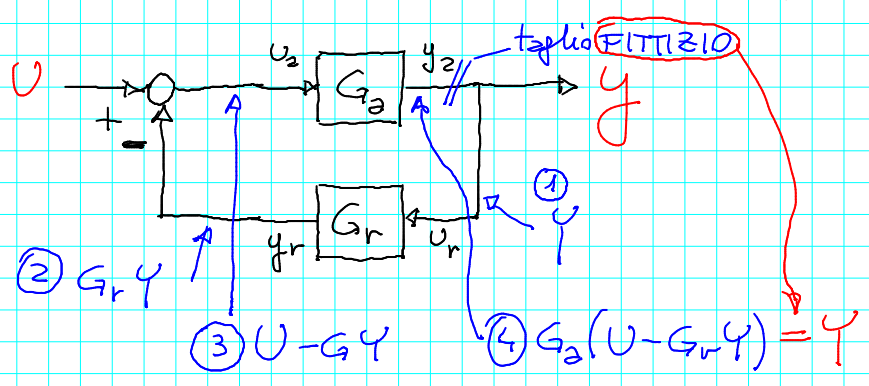
\includegraphics[height=5cm]{../lezione11/img5.PNG}
\end{center}
$G_a$ è il blocco di andata, mentre $G_r$ è il blocco di retroazione.\newline
Per capire come calcolare $\frac{Y}{U}$ immagino di tagliare l'anello nel punto di "taglio fittizio" dell'immagine. Seguiamo poi i numeri ($1-2-3-4$) nell'immagine per capire quanto valgono i vari segnali. Una volta arrivati al quarto punto, ripristiniamo il taglio fittizio e quindi possiamo porre $G_a(U-G_r Y) = Y$. Quindi rielaborando:
\[
    G_a U = (1+G_aG_r)Y \Longrightarrow \frac{Y}{U} = \frac{G_a}{1 + G_a G_r} \;\;\;\text{per ricordare si dice $\frac{\text{"andata"}}{1+ \text{"anello"}}$}
\]
Posti $G_a = \frac{N_a}{D_a}$ e $G_r = \frac{N_r}{D_r}$
\[
    \Longrightarrow \frac{Y}{U} = \frac{\frac{N_a}{D_a}}{1 + \frac{N_aN_r}{D_aD_r}} = \frac{\cancel{D_a}D_r \frac{N_a}{\cancel{D_a}}}{D_aD_r + N_aN_r}=
\]
questa elisione non è una cancellazione, nel senso che non porta a una parte nascosta, perchè è lo stesso polinomio che compare due volte e si elide nel calcolo, mentre per avere una cancellazione c'è bisogno che l'elisione avvenga fra polinomi diversi
\[
    = \frac{N_aD_r}{D_aD_r +N_aN_r}
\]
tra poli di $G_a$ e $G_r$ e gli autovalori del sistema complessivo non c'è una relazione banale:
\begin{itemize}
    \item $G_a$ e $G_r$ asintoticamente stabili nè occorrono nè bastano per avere un sistema complessivo asintoticamente stabile. (Dubbio proveniente dall'esercitazione 6 (lezione 16), esercizio 6: non ho ben capito il caso in cui si ha un blocco qualsiasi $G_1$ in parallelo (o in serie) a un anello $G_a$ composto da altri "sottoblocchi" (quello di andata e quello di ritorno)\dots chi deve essere asintoticamente stabile? Immagino che affinchè il sistema complessivo sia asintoticamente stabile, sicuramente $G_1$ dovrà esserlo (vedi proprietà dei blocchi in parallelo e in serie), ma per quanto riguarda l'anello $G_a$ complessivo, i suoi "sottoblocchi" non hanno nessun vincolo, in quanto non limitano la asintotica stabilità dell'intero anello $G_a$\dots Non sono sicuro al $100\%$, ma mi sembra un ragionamento sensato, TODO).
    \item possono esserci cancellazioni, cioè parti nascoste.
\end{itemize}
\ \newline
Vediamo questo ragionamento applicato allo spazio di stato:\newline
Equazioni costituitive dei blocchi:
\[
    G_a : (A_a, b_a, c_a,d_a); \;\;\;\;\;\;\;\;\;\;\;\;\;\;\; G_r : (A_r, b_r,c_r,d_r).
\]
Almeno uno dei due sistemi strettamente proprio è condizione sufficiente perchè l'anello sia ben posto, cioè le equazioni che conducono al sistema complessivo ammettono soluzione.\newline
Equazioni di connessione:
\[
    y = y_a; \;\;\;\;\;\;\;\;\;\; u_r = y_a \;\;\;\;\;\;\;\;\;\; u_a = u - y_r
\]
Di conseguenza:
\[
    \begin{cases}
        \dot{x}_a &= A_a x_a + b_a u_a = A_a x_a + b_a u - b_a y_r = A_a x_a + b_a u - b_a c_r x_r\\
        \dot{x}_r &= A_r x_r + b_r u_r = A_r x_r + b_r(c_ax_a + d_au_a) = A_r x_r + b_rc_ax_a + b_r d_a (u-c_rx_r) =\\
         &= A_r x_r + b_r c_a x_a + b_r d_a u - b_rd_ac_rx_r\\
        y &= t_a = c_ax_a + d_au_a = c_a x_a + d_a(u-c_rx_r) = c_ax_a + d_a u - d_a c_rx_r
    \end{cases}
\]
Che ci danno sistema matriciale:
\[
    \begin{cases}
        \left[\begin{matrix}
            \dot{x}_a\\\dot{x}_r
        \end{matrix}\right] = \left[\begin{matrix}
            A_a & -b_ac_r \\ b_rc_a & A_r-b_rd_ac_r
        \end{matrix}\right] \left[\begin{matrix}
            x_a\\x_r
        \end{matrix}\right] + \left[\begin{matrix}
            b_a \\b_rd_a 
        \end{matrix}\right] u\\
        y = \left[\begin{matrix}
            c_a & -d_ac_r
        \end{matrix}\right] \left[\begin{matrix}
            x_a\\x_r
        \end{matrix}\right] + d_a u
    \end{cases}
\]